% Fig 1b Circuit pic
\FloatBarrier

\begin{figure}[h!]
	\centering
	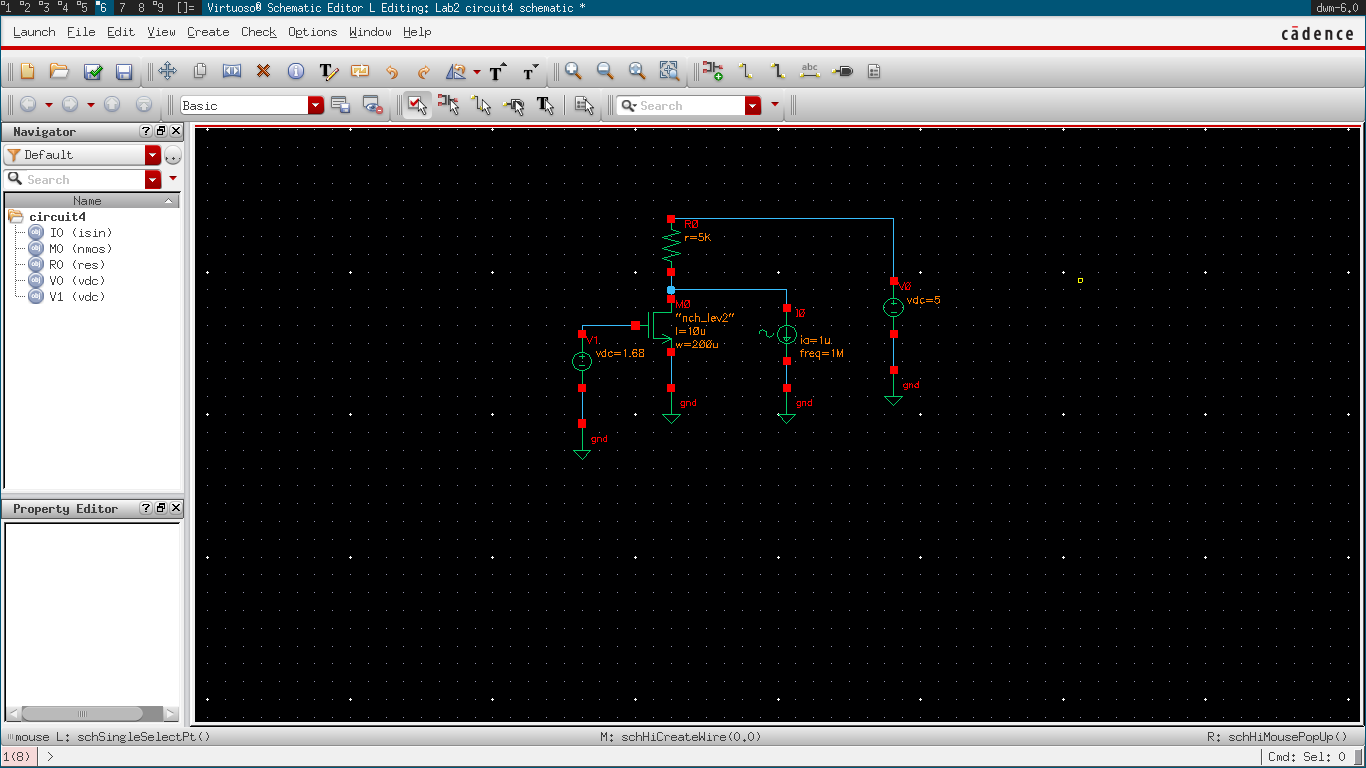
\includegraphics[scale=0.45]{../images/circuit4.PNG}
	\caption{Circuit 3}
	\label{fig:circuit3}
\end{figure}

\FloatBarrier
% Vx transient sim
The amplitude $V_{x}$ can be acquired by analyzing the results of a transient simulation.

\FloatBarrier

\begin{figure}[h!]
	\centering
	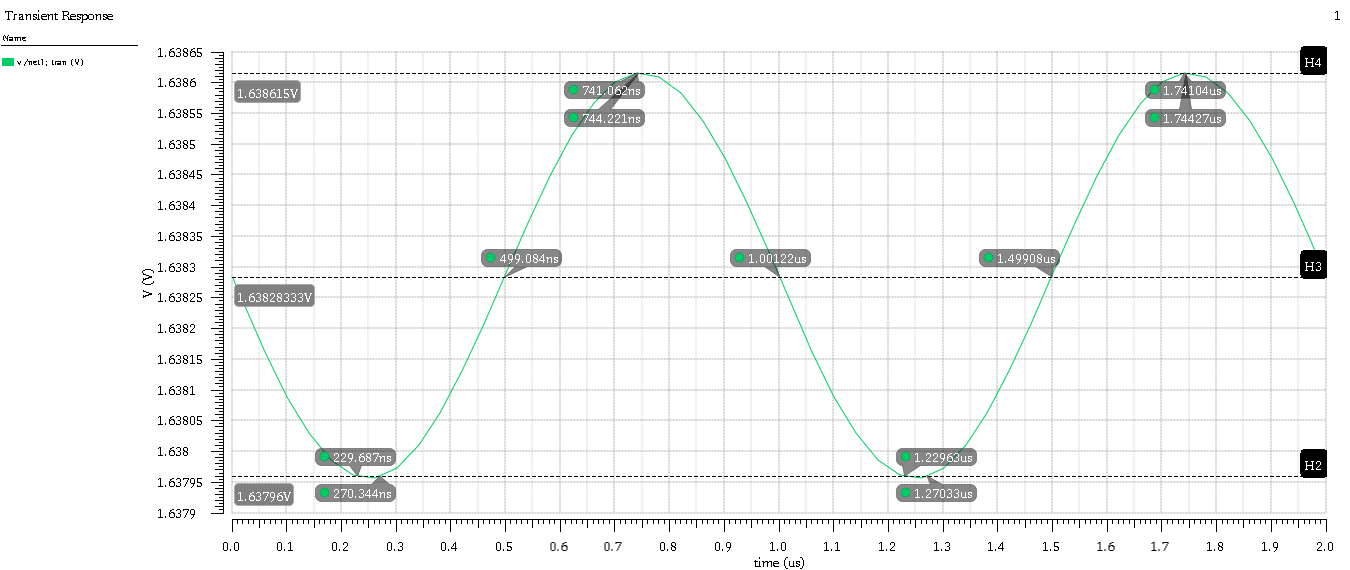
\includegraphics[scale=0.45]{../images/sim3_vx.PNG}
	\caption{$V_{x}$ Plot for Circuit in Figure (\ref{fig:circuit3})}
	\label{fig:sim3_vx}
\end{figure}

\FloatBarrier

% Calculate r_out. Once with equation and once with numbers. Compare with error.
The output resistance can be calculated simply by observing the amplitude of the waveform in figure (\ref{fig:sim3_vx}), also known as $V_{x}$, and dividing it by the input current amplitude, which is $1$\si{\micro\ampere} in this case.
The output resistance can be theoretically calculated for a common-drain amplifier using $r_{out} = R_{s} || \frac{1}{g_{m}} || r_{o}$.
Here, assume $r_{o}$ to be rather large.
Thus, the simplified expression $r_{out} = R_{s} || \frac{1}{g_{m}}$ is used for a theoretical comparison instead.
Clearly, the experimental result is consistent with theory.

\FloatBarrier

\begin{table}[h!]
	\centering
	\caption{$r_{out}$ for the Common Drain Amplifier}
	\label{tab:common_drain_amp_rout}
	\csvautotabular{../tables/common_drain_amp_rout.csv}
\end{table}

\FloatBarrier

% Fig 2b Circuit pic

\FloatBarrier

\begin{figure}[h!]
	\centering
	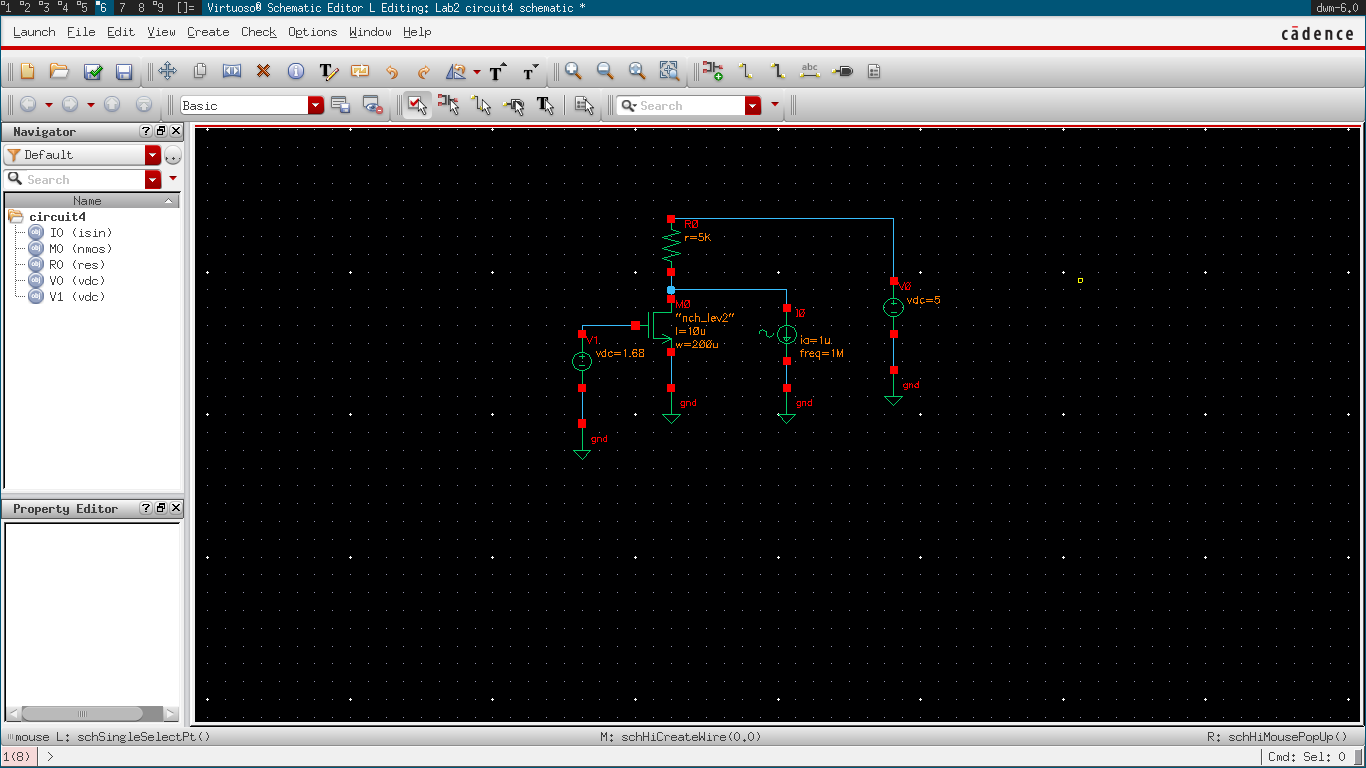
\includegraphics[scale=0.45]{../images/circuit4.PNG}
	\caption{Circuit 4}
	\label{fig:circuit4}
\end{figure}

\FloatBarrier
% Vx transient sim

\FloatBarrier

\begin{figure}[h!]
	\centering
	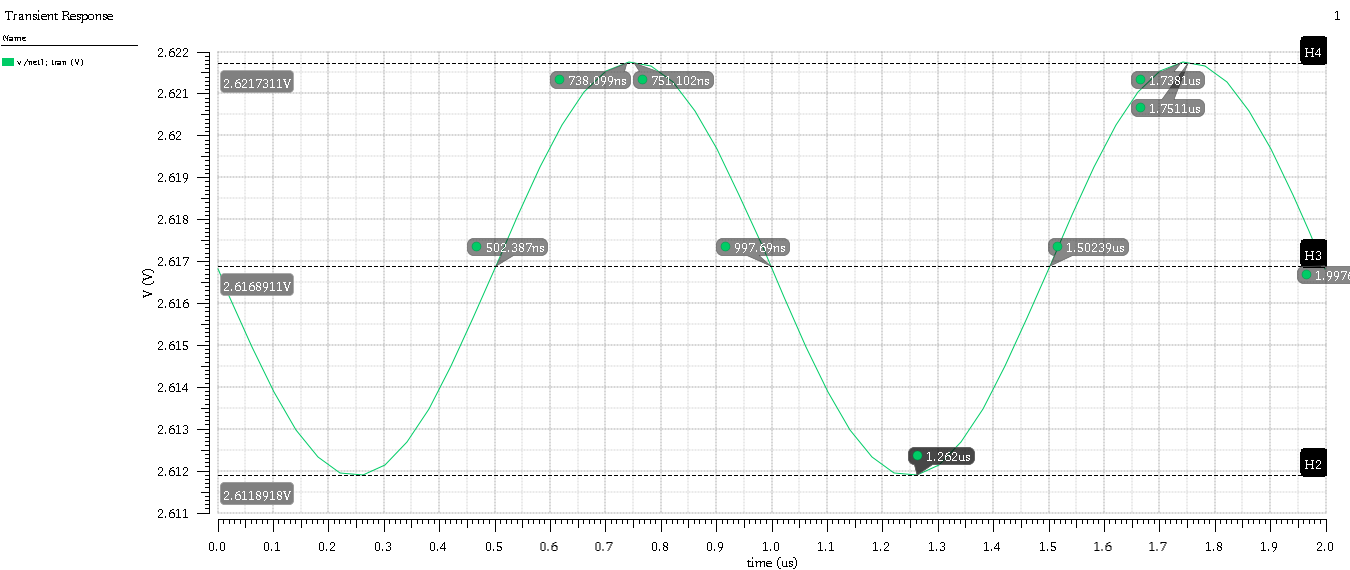
\includegraphics[scale=0.45]{../images/sim4_vx.PNG}
	\caption{$V_{x}$ Plot for Circuit in Figure (\ref{fig:circuit3})}
	\label{fig:sim4_vx}
\end{figure}

\FloatBarrier
% Calculate r_out. Once with equation and once with numbers. Compare with error.

\FloatBarrier

\begin{table}[h!]
	\centering
	\caption{$r_{out}$ for the Common Drain Amplifier}
	\label{tab:common_source_amp_rout}
	\csvautotabular{../tables/common_source_amp_rout.csv}
\end{table}

\FloatBarrier
From these results, it is clear that the common-drain amplifier has a much lower output resistance.
